% !TeX spellcheck = it_IT
\section{Due esempi di corollari}

% --- Il teorema di Chow e Gulliver ---
\begin{frame}{Due corollari}{}
	\begin{block}{Corollario (Chow)}<1->
		Data una soluzione $C^2$ al problema, esiste $C$, \textbf{che dipende solo dal dato iniziale}, tale che ad ogni istante $t$:
		\begin{equation}
			\max_{x\in X_t} |x| - \min_{x\in X_t} |x| <C
		\end{equation}
	\end{block}
	\begin{block}{}<2->
		Se considero la soluzione riscalata, $\frac{X_t}{\max_{x\in X_t} |x|}$, per un flusso espansivo dove $\lim_{t\rightarrow T}\max_{x\in X_t} |x| = +\infty$, converge a una sfera 
	\end{block}
	\begin{block}{Corollario (Sinestrari)}<3->
		Non esistono soluzioni antiche espansive ($F<0$) che \textit{escono fuori da un punto} oltre alle sfere. 
	\end{block}
\end{frame}

\section{Cenni sull'estensione a spazi a curvatura costante}
% --- Frame: text and figure ---
\begin{frame}{Estensione a spazi a curvatura costante}{(idea)}
	\begin{columns}
		% First column
		\column{.5\textwidth}
		Il risultato di Chow e Gulliver si estende al caso in cui lo spazio ambiente è uno spazio a curvatura costante. 
		\begin{itemize}
			\item L'equazione continua ad essere parabolica anche negli spazi a curvatura costante
			\item Introduciamo una notazione che consente di impostare il problema
			\item La dimostrazione non utilizza la metrica, per cui può essere estesa		
		\end{itemize}
		% Second column
		\column{.5\textwidth}
		\begin{figure}
			\begin{center}
				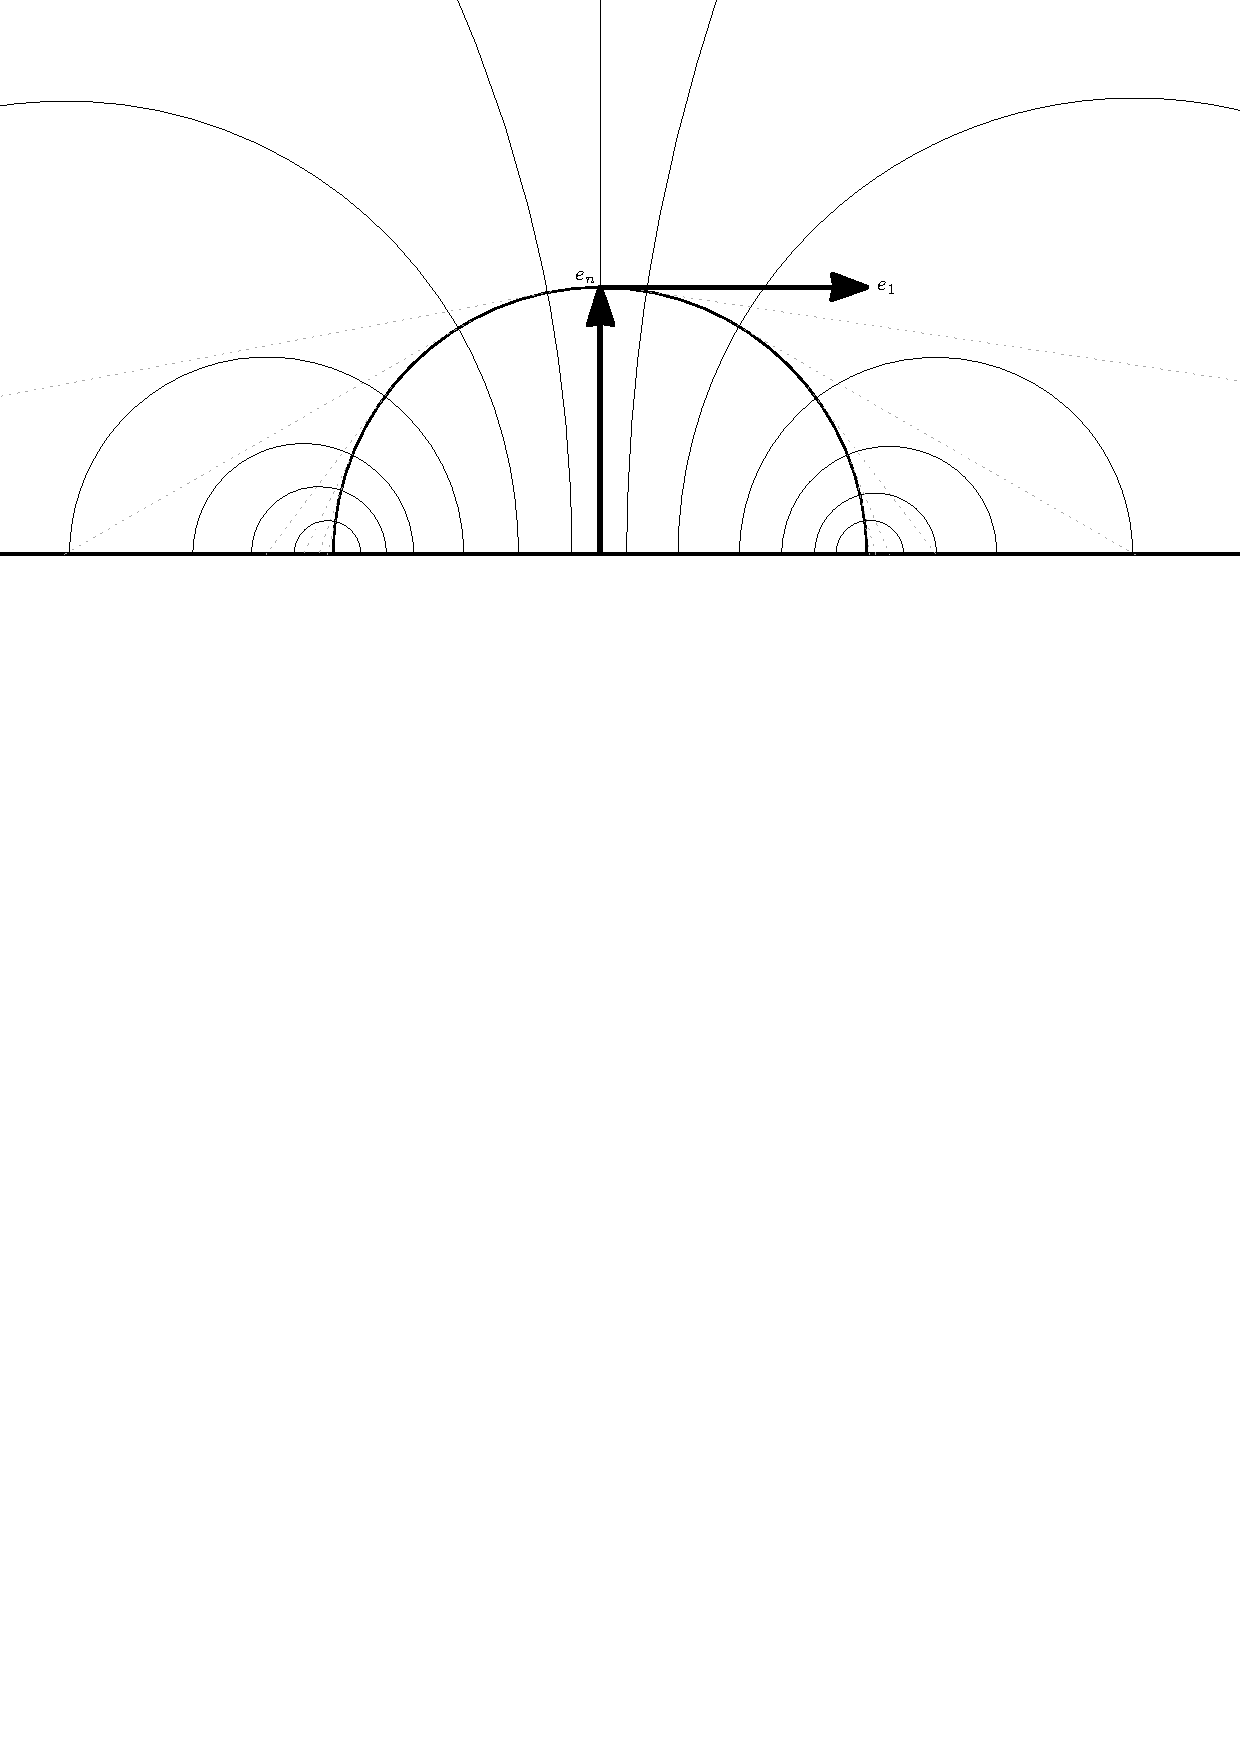
\includegraphics[width=\textwidth]{5b_moving_planes_hyperbolic}
				\caption{Iperpiani totalmente geodetici perpendicolari a una data geodetica in $\mathbb{H}^2$}
			\end{center}
		\end{figure}
	\end{columns}
\end{frame}
